In the last few years, there has been significant growth in grid-connected distributed energy resources (DERs) leading to an increased deployment of distributed generation (DG) and recently more distributed storage (DS) systems. Companies have started to heavily invest in the competitive energy storage system market by taking advantage of the decreasing costs of energy storage. Although a significant amount of DG and DS are being added to the distribution grid, need to improve their control systems for seamless integration to the grid is still there. In the US, most DG and DS systems are deployed to either help reduce the metered load through net-metering programs or to sell power to the utility through power purchase agreements (PPAs). The potential of DG combined with DS is not fully utilized under these pricing schemes due to the lack of proper control schemes. In order to maximize the use of available DERs, a state-of-the-art energy management solution is a necessity for our future smart grid. Such an energy management solution will be able to dynamically optimize the use of all the available DS with the objective of serving the load in the most economical and safe way possible. This will benefit both utility companies and regular consumers. Due to the constraints and intermittent nature of some DG systems, such as wind and solar, the optimum management of DS combined with a DG is a difficult problem to solve. The most common approaches found in the current literature are as follows. Some researchers formulate the problem as a linear programming (LP) or mixed integer linear programming (MILP) model \cite{lp73, lp74, lp75}. Authors in \cite{pso80, pso81} present an energy management solution based on particle swarm optimization for a microgrid containing wind turbines and energy storage (ES) system. Other researchers propose crow-search and ant colony optimization models to solve the energy management problem for local microgrids as seen in \cite{csa87} and \cite{aco84}. There have also been model predictive control (MPC) based approaches for managing ES in microgrid settings as seen in \cite{energymanajaboulay,mpcmorstyn}.  Researchers in \cite{ga76, ga77} have also proposed genetic algorithm based solutions to optimize the ES operation in a microgrid. One clear disadvantage of these proposed models is that most of these approaches only consider the current status of the system and ignore some critical factors like energy tariff, forecasted load, and forecasted generation profiles.  These information can be used to find an optimum solution based on both current and probable future states of the system as opposed to a solution relying only on the currently available data. Off-line day ahead planning models have also been proposed in the literature. In these methods, available predicted data is used to optimize the scheduling of the ES based on Monte Carlo simulations \cite{6872821,7010943,6839110}. These solutions are very computationally intensive and require a lot of time for planning the day ahead. The computational complexity makes them unsuitable for real-time implementation. Also, as they are based on off-line calculations and rely vastly on the accuracy of the predictions.

From the discussion thus far, it is evident that there is a need for a real-time ESM solution that can optimize the long-term operating costs of a system containing DG and an energy storage (ES) system. This paper presents an optimum real-time control strategy for such systems. The proposed control strategy takes into account the present and forecasted states of the system, together with the real-time price (RTP). The rest of the paper is organized as follows.



\section{Problem formulation} \label{formulation}
In this section the problem of optimizing the energy store based on current and forecusted data is formulated. Fig. \ref{fig:system_arch} depicts an example system. Here, the energy storage management system (ESMS) is in charge of controlling the battery connected to the grid with the objective of getting the most cost optimum use of the resources available. The objective of the ESMS is to optimize the use cost of energy storage under different pricing schemes by taking advantage of RTP or time of use (TOU) prices, load and DG generation forecasting.  Fig. \ref{fig:F1_CA} shows the top-level architecture of the ESMS. As seen in the figure, the inputs of the system are the real-time price (RTP) prediction, load prediction, and the DG output prediction, which in this case is a photovoltaic (PV) plant output. It will also consider the current state of the load, current PV generation, and the state of charge of the ES. The output of the ESMS is the optimum battery charge and discharge control references based on the current and forecasted data.

\begin{figure}[!htbp]
\centering
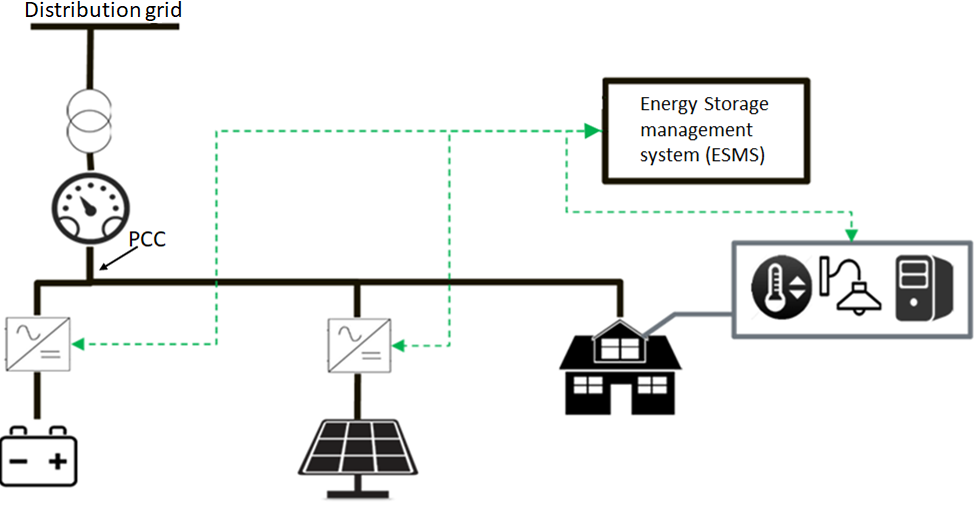
\includegraphics[width=0.6\linewidth]{figs/A8/System_architecture.png}
\caption{Example test system architecture}
\label{fig:system_arch}
\vspace{-3mm}
\end{figure}

%  Fig. \ref{fig:F1_CA} shows the top-level architecture of the ESMS. As seen in the figure, the inputs of the system are the real-time price (RTP) prediction, load prediction, and the DG prediction, which in this case is a photovoltaic (PV) plant. It will also consider the current state of the load, PV generation, and ES. The output of the ESMS is the optimum battery charge and discharge control references based on the current and forecasted data.

\begin{figure}[!ht]
    \centering
    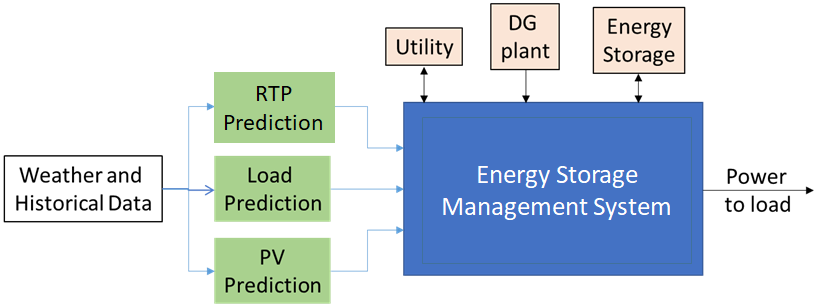
\includegraphics[width = 0.8\linewidth]{figs/A8/EMS_FIG.png}
    \caption{Controller top level architecture}
    \label{fig:F1_CA}
\end{figure}

Determining the optimum reference for the ES in continuous domain is a difficult and computationally intensive tusk. To make the problem solvable is a fast manner the solution space of the problem is discretized. Fig. \ref{fig:F1_Dis} demonstrates an example of the discretized solution space. The horizontal axis of the figure represents time, and the vertical axis represents discrete steps in the state of charge (SOC) of the energy storage. The solution space in the figure assumes that forecast data for the next 45 minutes are available and a control action is taken every 15 minutes. The SOC of the ES is limited between 80\% and 20\%. It is also assumed that the ES can discharge a maximum of 40\% of its maximum SOC and charge a maximum of 20\% of its SOC in a 15 minutes. The space between the upper and lower bounds of the SOC is discretized in steps of 20\%. This allows us to define the solution space as a directional graph. In the graph represented in the figure a discrete value of SOC at a discrete time is a node or a vertex. The possible paths from one node to another node at the next  time step can be defined as a directional edge. Using these definitions the solution space can be defined as a directional graph. The parameters chosen for this simple example are arbitrary. A similar graph can be constructed for various situations based on system properties and constraints.

% In order to find the optimum cost solution based on the current status of the system and future forecasts, the optimization problem is formulated using a graph search problem approach. To represent the solution space of the problem as a graph, the state of charge (SOC) of the ES, and both the prediction horizon and the control horizon are discretized. Fig. \ref{fig:F1_Dis} demonstrates an example of the discretized solution space.
\begin{figure}[!ht]
    \centering
    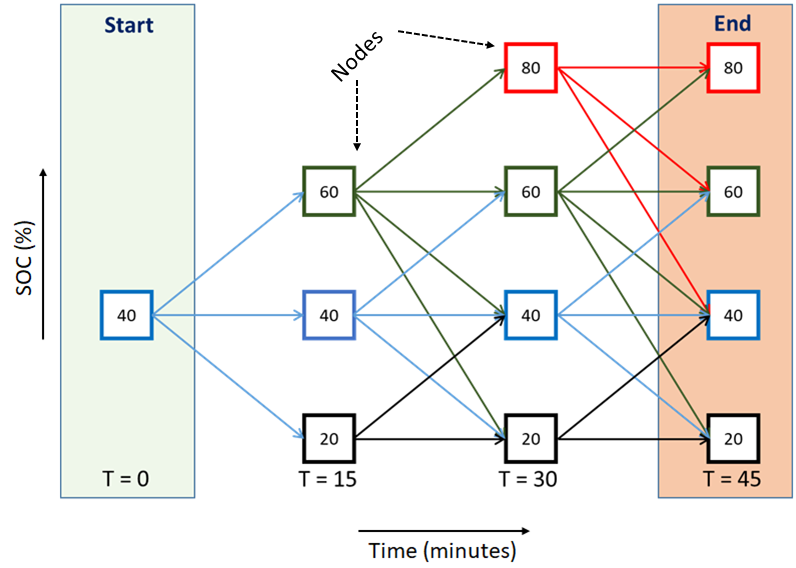
\includegraphics[width = 0.6\linewidth]{figs/A8/F1_1_Dis.png}
    \caption{Discretizing solution space}
    \label{fig:F1_Dis}
\end{figure}

% The horizontal axis of the figure represents time, and the vertical axis represents discrete steps in the state of charge (SOC) of the energy storage. In this simple example scenario, it is assumed that the algorithm recalculates the solution every 15 minutes (control horizon) based on available data. The SOC of the energy storage system (ESS) is discretized in steps of 20\%, and the SOC is limited between 80\% and 20\%. It is also assumed that the ESS can discharge a maximum of 40\% of its maximum SOC and charge a maximum of 20\% of its SOC in a 15 minute time step. These values are chosen arbitrarily in this simple example scenario to explain the problem. Taking these features into consideration, a directed graph is constructed looking ahead three-time steps into the future. The square boxes represent nodes on the graph. The numbers inside the boxes represent the SOC of the ESS at that node. The arrows from the boxes represent all the possible states the ESS can be in the next time step according to the constraints of the system. The arrows are treated as edges of the graph. In this case, the edges are unidirectional. The goal is to find the most cost-efficient path to reach T = 45 minutes. Although in this example the algorithm considers T = 45 as the final stage, in actual application the final stage can be determined based on the actual use case.

\section{A* based energy management system} \label{A*}

\subsection{A* Search Algorithm}
A* is a computer algorithm which is widely used to solve graph search problems \cite{a8book}. It determines the most efficient path between multiple nodes in a graph. A* is an informed search algorithm. This means, it searches between all the possible paths to the goal and finds the path incurring the least cost. To do this, it considers the paths which appear to have the least cost to get to the goal first. Starting from a specific node, it explores the graph step by step depending on the cost of going from one node to the next. The algorithm selects the node to explore based on a combination of the actual cost to get to the node and a heuristic cost that estimates the cost from the current node to the goal. The process to calculate heuristic cost is problem-specific. For the algorithm to work correctly, the heuristic cost has to be less than or equal to the actual cost of getting to the goal node. In other words, the heuristic cost function should never overestimate the cost of reaching the goal. The algorithm works by calculating the combined actual and heuristic cost for all the neighboring nodes of the starting node and puts them into a priority queue called the \textit{open list}. Then, it selects the node with the least cost and expands that node to get the cost of its neighbors. The expanded node is taken out of the priority queue and put in another list called the \textit{closed list}. The algorithm continues to expand the \textit{open list} always selecting the node with the least cost and adding it to the \textit{closed list}. The algorithm terminates when the goal node is inside the \textit{open list}, and it has the minimum cost in the \textit{open list}. Finally, the algorithm retraces its path through the \textit{closed list} to find the optimum route from start to goal. Pseudo code for the A* algorithm is given below.

\textbf{Algorithm 1:} A* search algorithm

\begin{algorithmic}[1]
\label{al:1}
% \Function{heuristic\_estimate}{$a,b$}
%     \State $hCost := \sum_{n=a}^b D(n)*R_{best}(n) $
%     \State \Return $hCost$
% \EndFunction

% \Function{gCost\_calc}{$p,c$}
%     \State $C_{actual}(pc) := C_{ESS}(pc)+C_{GRID}(t)+C_{best}(p)$
%     \State \Return $C_{actual}(pc)$
% \EndFunction

\Function{A*}{$start, goal$}
\State $Closed\_Set = \{\}$ \Comment{Set of evaluated nodes}
\State $Open\_Set = \{Start\}$ \Comment{Set of already discovered nodes which have not been evaluated. Initially,  the start node is discovered.}
\State $Best\_Parent[Start] = \{ \}$ \Comment{It is the node from which the current node can be most effectively reached. At initialization it is empty because the start node has no parent node.}
\State $F\_cost[Start] = G\_cost[Start] + H\_cost[Start]$ \Comment{$F\_cost$ is the combination of the actual cost of reaching a node from the start node \& the heuristic cost of reaching the goal node from the current node. $G\_cost$ is the actual cost \& $H\_cost$ is the heuristic cost of the current node. the Start node has a $G\_cost$ of $0$.}
\While{$Open\_Set$ is not empty}
    \State $Current\_Node = $ node in $Open\_Set$ with lowest $F\_cost$
    \If{$Current\_Node$ == goal}
      \State  \textbf{break} 
    \EndIf
    \For {Each child node of $Current\_Node$}
        \If{Child node in $Closed\_Set$}
            \State \textbf{continue}
        \EndIf
        \If{Child node in $Open\_Set$}
            \If{$G\_cost[child]$ $\geq$ $G\_cost$ already in $Open\_Set$}
                \State \textbf{continue}
            \EndIf
        \EndIf
        \State $Best\_Parent[child] = Current\_Node$
        \State $F\_cost[child] = G\_cost[child] + H\_cost[child]$
        \State $Open\_Set.add(child)$ \Comment{Add child node to $Open\_Set$}

    \EndFor
    \State $Closed\_Set.add(Current\_Node)$ \Comment{Add $Current\_Node$ to $Closed\_Set$}
    \State $Open\_Set.remove(Current\_Node)$ \Comment{Remove $Current\_Node$ From $Open\_Set$}
\EndWhile
\State $Best\_Path = \{ \}$ \Comment{$Best\_Path$ is the most efficient path to get to the goal node.}
\While{$Best\_Parent[Current\_Node] != \{ \}$}
    $Current\_Node = Best\_Parent[Current\_Node]$
    $Best\_Path.add(Current\_Node)$ \Comment{Add $Current\_Node$ to $Best\_Path$}
\EndWhile
\State \Return $Best\_Path$
\EndFunction
\end{algorithmic}

The steps of the algorithm and how it works is explained with a simple example in Fig. \ref{fig:A_STAR_EXAMPLE}. The nodes with white background are the unexplored nodes. The Nodes with orange background are the nodes in open list and nodes with gray background are the nodes in the closed list. The black arrows shows the edges of the graph and the numbers on them represents the cost of taking the edge. The dotted red lines represent heuristic costs from a node to the goal node and their values are represented by the red numbers. The graph shown in the figure is represented as
\begin{equation}
    Z = ( V(Z), X(Z) )
\end{equation}
Here, $V$ is the set of nodes or vertices and $X$ is the set of ordered pairs or edges used the represent the graph Z. Their elements are shown in (\ref{eq:V_Z}) and (\ref{eq:X_Z}) respectively.
\begin{equation}
\label{eq:V_Z}
    V(Z) = \{A,B,C,E,F,G,H\}
\end{equation}
\begin{equation}
\label{eq:X_Z}
    X(Z) = \{ (A,B), (B,E), (E,H), (A,C), (C,G), (C,F), (F,H) \}
\end{equation}

The goal here is to start at node A of Z and find the shorted path to reach node H. In the beginning, Algorithm 1 is given the start node A and goal node H. Then at line 2 the algorithm initializes an empty $Closed\_Set$. Then it initializes the $Open\_Set$ with the starting node which is A in line 3. Then the $F\_cost$ of node A is set to $\infty$ at line 4. These steps are represented in Fig.\ref{fig:A_STAR_EXAMPLE}(a).  Then we enter the while loop in line 5 of the algorithm. As the open set contains the node A the loop continues. On line 6 $Current\_node$ is set to A as A is the only node in open set. Now as $Current\_node$ is not H (goal node) we continue to line 10 of the algorithm. Here, for each child node of $Current\_node$ the algorithm first checks if the node is in closed set. If the child node is in $Closed\_set$ the child node is ignored. Then on lines 14 \& 15 the algorithm checks if the child node is in $Open\_set$ and is the $G\_cost$ of getting to the child is higher than the $G\_cost$ currently present in $Open\_Set$ then the child is ignored. Otherwise we continue with the algorithm and in line 19 the $Current\_Node$ is set as the best parent of the child node. Then the $F\_cost$ of the child node is calculated by adding the $G\_cost$ and $H\_cost$ of the child in line 20. Then the child is added to the $Open\_set$ in line 21. After that in line 23 and 24 of the algorithm the current node is added to the $Closed\_Set$ and taken out of the $Open\_Set$. In the example shown in Fig. \ref{fig:A_STAR_EXAMPLE}, the two children B \& C of node A are explored in this step. As none of them are in $Open\_Set$ or $Closed\_Set$ we calculate the their F costs and add them to the $Open\_Set$. Also node A is taken out of the $Open\_Set$ and added to the $Closed\_Set$. These changes can be noticed in Fig. \ref{fig:A_STAR_EXAMPLE}(b). The gray background behind node A represents that it is in the closed set and the orange backgrounds behind nodes B and C represents they are in the $Open\_Set$. Now the algorithm goes back to line 5 and as $Open\_Set$ is not empty it continues on. This time the node with the lowest cost is B so the children of B are explored. Which reveals the new node E which is added to the $Open\_Set$ and B is taken out of the $Open\_Set$ and added to the $Closed\_Set$. This brings us to the state of the search shown in Fig. \ref{fig:A_STAR_EXAMPLE}(c). $Open\_Set$ not empty so the algorithm continues and chooses node E as current node as it has the lowest $F_Cost$ in the $Open\_Set$. This leads to the discovery of node H which is our goal node. H is added to the $Open\_Set$. E is taken E is taken out of the $Open\_Set$ and added to the $Closed\_Set$. These steps are reflected on Fig. \ref{fig:A_STAR_EXAMPLE}(d). Now we have a path to H and H is the node with the smallest F cost in the $Open\_Set$. SO the algorithm exits the while loop on line 8 and continues to line 26. here best path is initialized as and empty set. Then the algorithm traces back the $Best\_Parent$ of the $Current\_node$ in the while loop between lines 27 to 30 in the algorithm until it reaches the start node. And that gives us the $Best\_Path$. This is shown in Fig. \ref{fig:A_STAR_EXAMPLE_2}. In this case the best path from A to H is A, B, E \& H. This path is shown by the nodes highlighted in blues in the figure.

\begin{figure}[!ht]
    \centering
    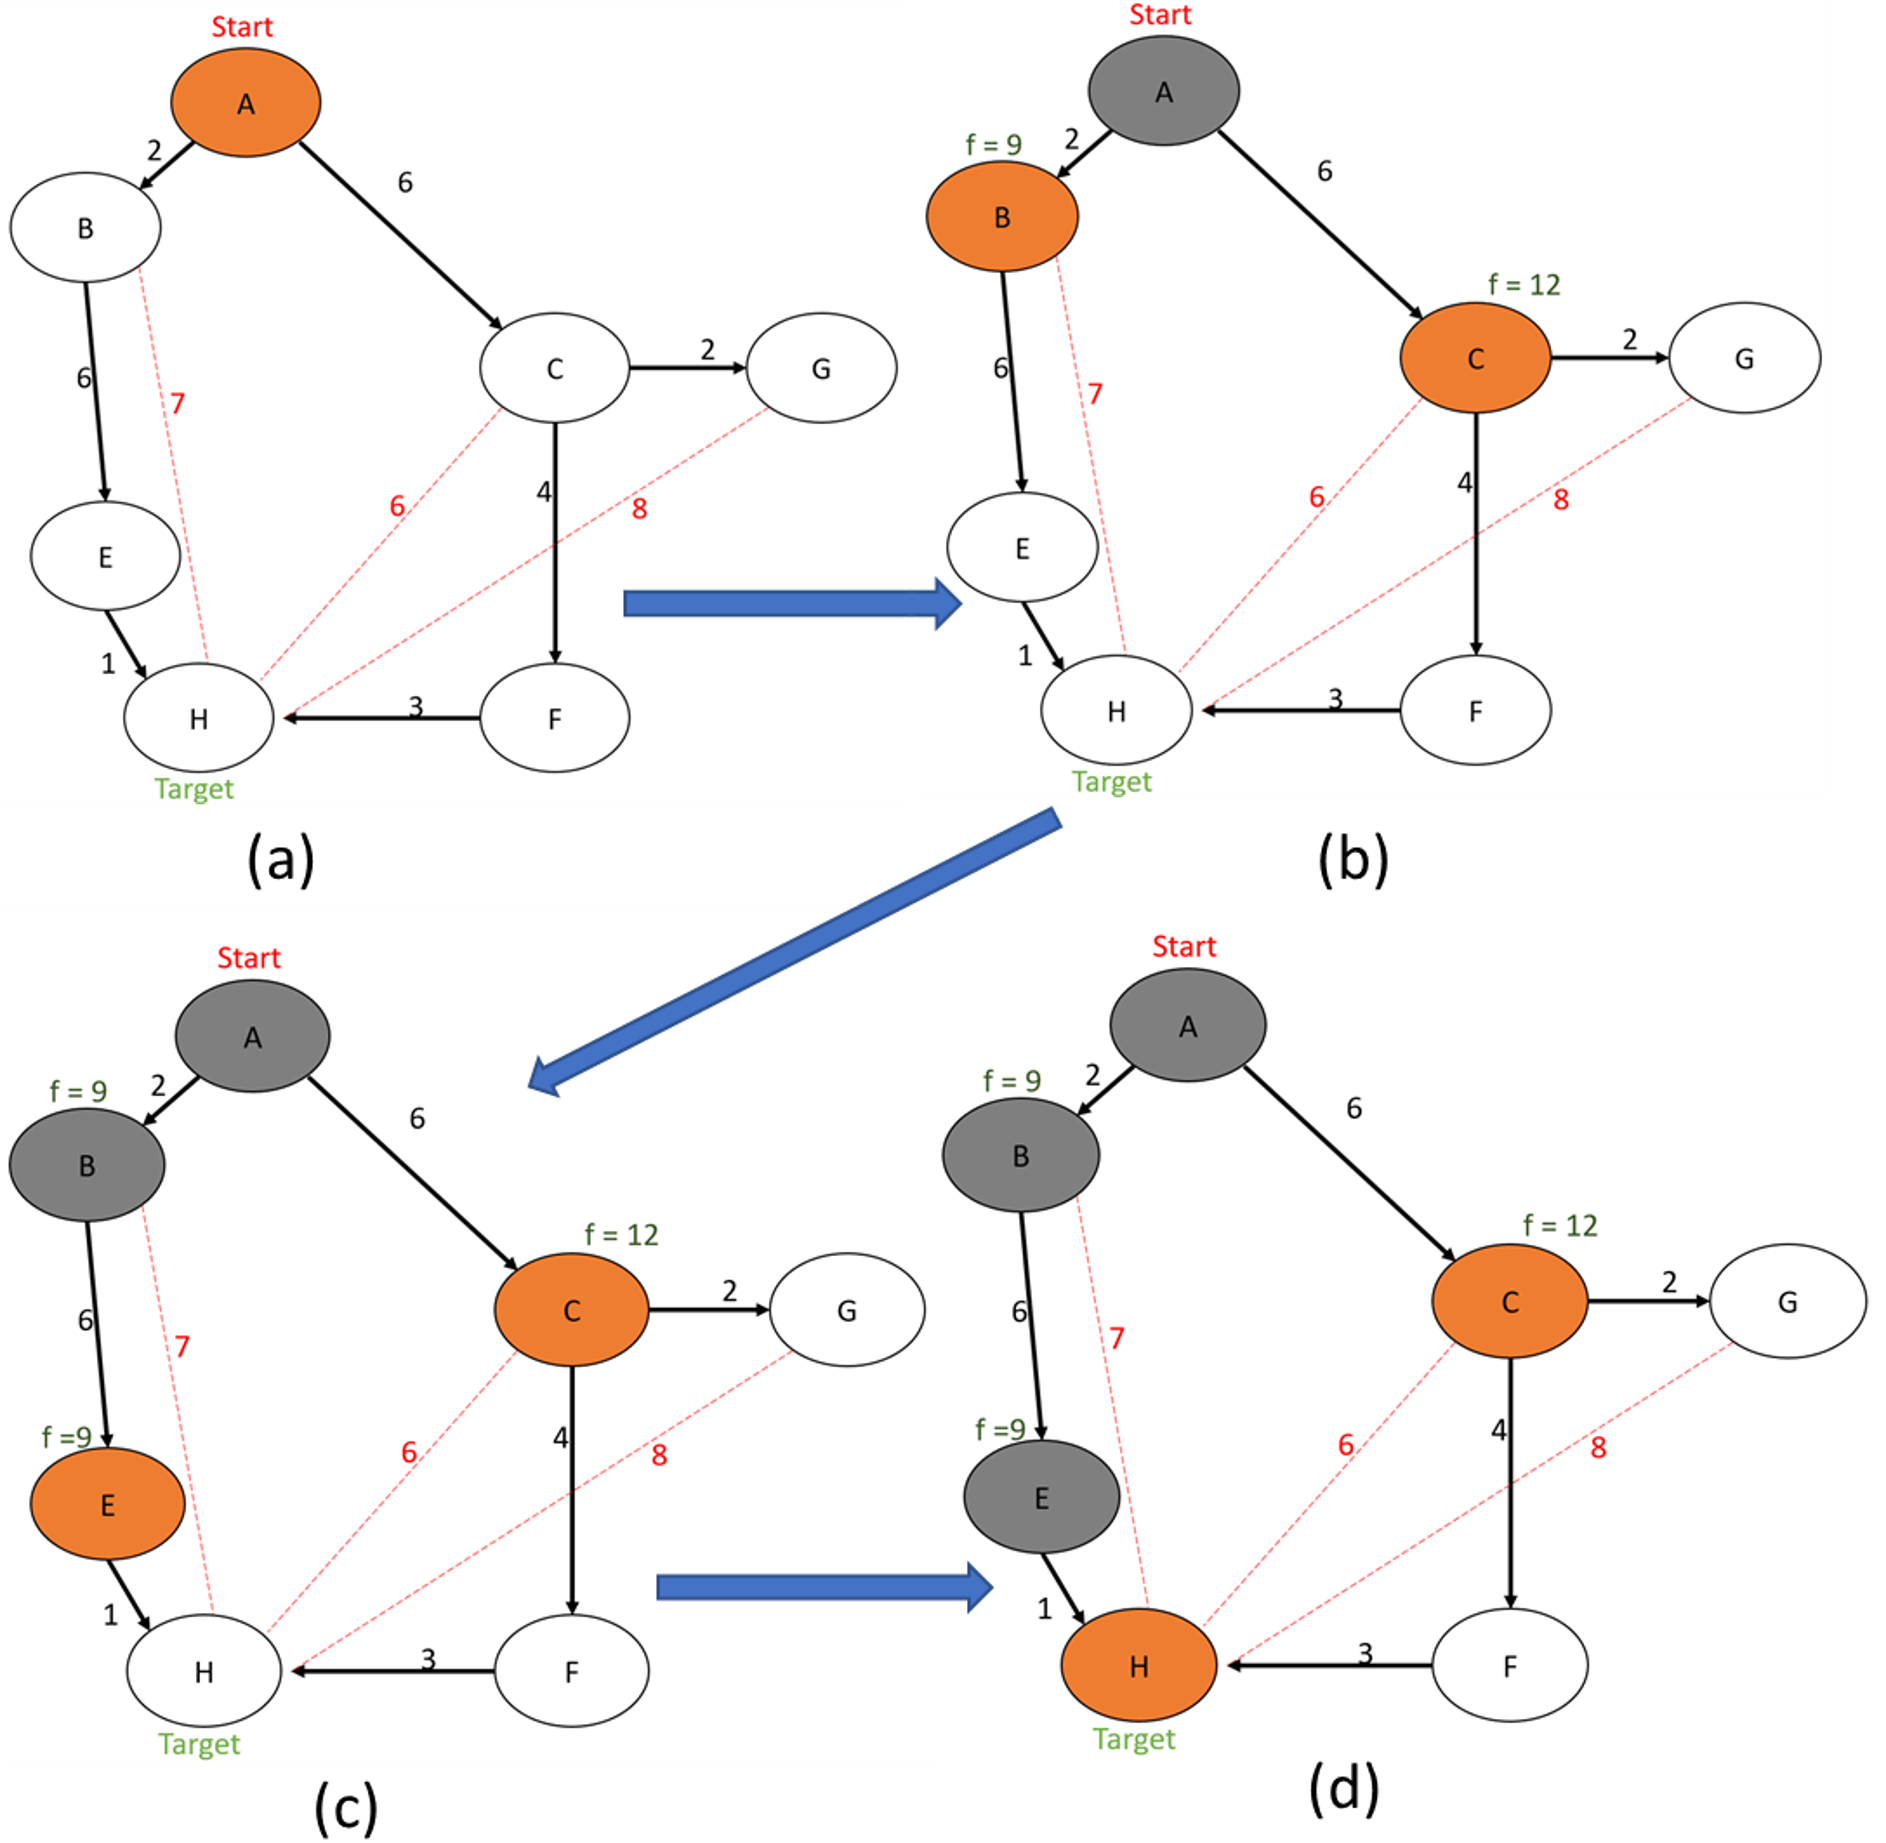
\includegraphics[width = \linewidth]{figs/A8/A_STAR_EXAMPLE.png}
    \caption{A* path finding example to find the shortest path between the nodes A and H of graph Z.}
    \label{fig:A_STAR_EXAMPLE}
\end{figure}


\begin{figure}[!ht]
    \centering
    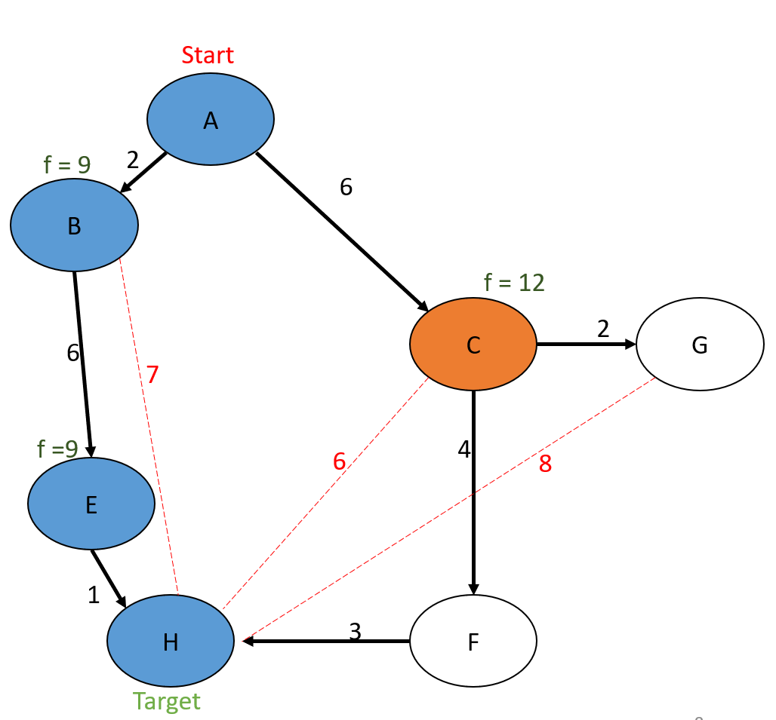
\includegraphics[width = 0.5\linewidth]{figs/A8/A_STAR_EXAMPLE_2.png}
    \caption{A* path finding example best path from A to H.}
    \label{fig:A_STAR_EXAMPLE_2}
\end{figure}


% Fig. \ref{fig:A_STAR_PIC} shows an example of the A* algorithm in a simple directional graph. The capital letters A, B, C, E, F, G and H inside the ellipses represent the nodes of the graph. The starting point of the graph is A, and the goal is to find the shortest path to node H. The solid blue arrows indicate the directional path from one node to the next. The actual cost of taking these paths are represented by the blue numbers beside the solid blue arrows. The red dotted lines represent the heuristic costs from a node to the target (goal) node. The heuristic costs of nodes B, C and G are shown as 7, 6 and 8. The letter 'h' is used to denote this cost. The algorithm starts at node A and discovers the surrounding nodes B and C. The combined heuristic and actual cost of node B is 9 and it is denoted by the letter 'f'. The 'f' cost for node C is 10. So, the algorithm will choose node B as the main candidate to explore. In node B, node E is discovered to have a combined cost of 10. Now, between the nodes C and E, the algorithm will choose a node at random. In this case, let us assume the node selected by the algorithm is E. After expanding E, the algorithm will find a path to node H which costs 10. However, this is still not the lowest path cost among all the nodes in the priority queue. C also has a cost of 10. So, the algorithm will expand the node C and discover two new nodes G and F. The combined heuristic and actual cost of node G is 15 and node F is 14, which in turn are more than 10. So, the algorithm will stop searching and decide that the shortest path from node A to H is the path previously discovered. By using this approach, A* lets us avoid exploring the nodes G and F because the combined heuristic and actual cost of a node are less than or equal to the actual cost taking a path through that node to the target.





% \begin{figure}[!ht]
% \centering
% %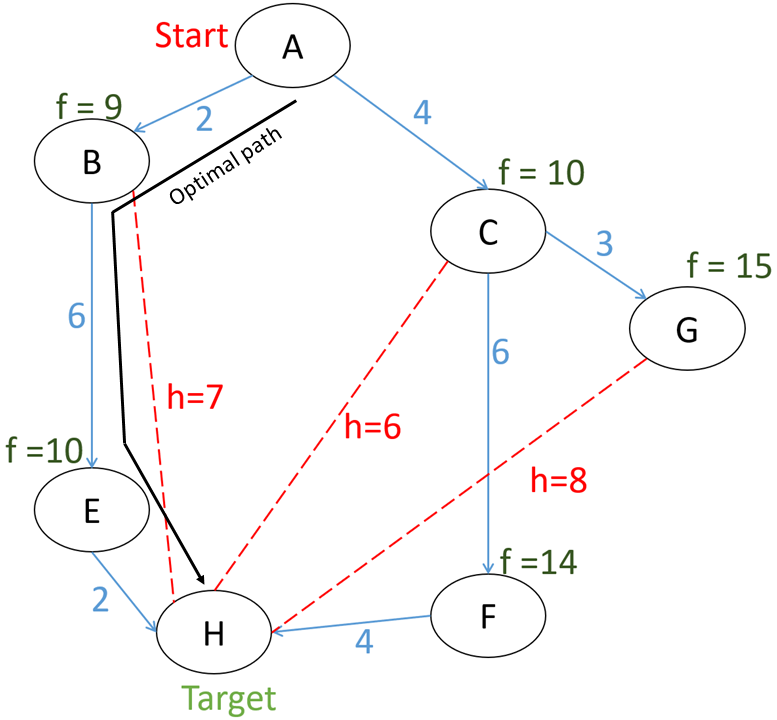
\includegraphics[width=\linewidth]{figs/A_STAR_PIC.png}
% 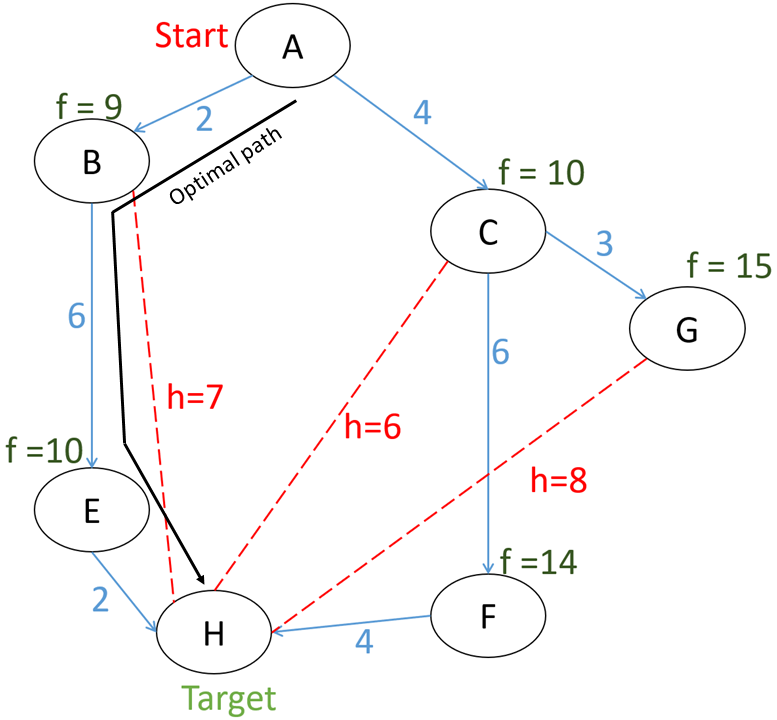
\includegraphics[width=\linewidth]{figs/A_STAR_PIC.png}
% \caption{Example graph for A* implementation}
% \label{fig:A_STAR_PIC}
% \end{figure}

\subsection{Implementation}
By defining the solution space with a combination of nodes and edges, the ESM optimization problem can be formulated as a graph search problem as well. At the inception, the starting node is determined by the current status of the system. Then, the following nodes and edges are generated using the forecasted data available. A discrete set of endpoints are set as the goals of the search. The A* algorithm stops when one of the endpoints are in the $Open\_Set$ and they have the lowest $F\_cost$. The cost of going from a parent node to a child node is calculated by combining the real cost of getting to that child node and the heuristic cost of getting to the goal from that child node. The real cost of going from a parent node $p$ at time $T=t$ to a child node $c$ at time $T=t+\Delta T$ is denoted as $C_{actual}(pc)$. It is calculated according to (\ref{eq:C_actual}).

\begin{equation}
\label{eq:C_actual}
    C_{actual}(pc) =  C_{ESS}(pc)+C_{GRID}(t)+C_{best}(p)
\end{equation}

Here, $\Delta T$ represents the time between two time steps. $C_{actual}(pc)$ represent the total cost of going to the child node $c$ from parent node $p$. $C_{ESS}(pc)$ represent cost of energy storage to go from parent node $p$ to child node $c$. $C_{GRID}(t)$ is the cost of using the grid between time $T=t$ and time $T=t+\Delta T$. $C_{best}(p)$ represent the best or least cost to get to the parent node $p$ from the start node. $C_{ESS}(pc)$ is calculated according to (\ref{eq:C_ESS}).

\begin{equation}
\label{eq:C_ESS}
C_{ESS}(pc) = |(SOC_p - SOC_c)|*ESS_{CAP}*R_{ESS} 
\end{equation}

Here, $SOC_p$ and $SOC_c$ represent the state of charge at parent and child node. $ESS_{CAP}$ represent the total energy capacity of the energy storage. And $R_{ESS}$ is the $\$/kWh$ cost of using the energy storage. $C_{GRID}(t)$ is calculated according to (\ref{eq:C_GRID}).

\begin{equation}
\label{eq:C_GRID}
C_{GRID}(t) = 
\begin{cases}
   E_{GRID}(t)*RTP(t),& \text{if } E_{GRID}(t)\geq 0\\
    E_{GRID}(t)*SP(t),& \text{if }  E_{GRID}(t) < 0
\end{cases}
\end{equation}

Here, $E_{GRID}(t)$ is the energy drawn from the grid between time $T=t$ and time $T=t+\Delta T$. $RTP(t)$ is the real-time price between $t$ and $t+\Delta T$. $SP(t)$ is the price the utility is willing to pay the consumer for selling power between $t$ and $t+\Delta T$. The heuristic cost is calculated by assuming that whichever source has the smallest cost during a time step will supply the total energy demand of that particular time step. The heuristic cost of a node at time $T = t$ is calculated according to (\ref{eq:C_H}).

\begin{equation}
\label{eq:C_H}
C_H(t) = \sum_{n=t}^{end} D(n)*R_{best}(n)
\end{equation}

Here, $C_H(t)$ represents the heuristic cost at time $t$. $D(n)$ is the demand between time $T = n$ and time $T = n+\Delta T$. $R_{best}(n)$ is the source with the smaller cost which is calculated according to (\ref{eq:R_best}).

\begin{equation}
\label{eq:R_best}
R_{best}(n) = 
\begin{cases}
    R_{ESS},& \text{if } RTP(n)\geq R_{ESS}\\
    RTP(n),              & \text{otherwise}
\end{cases}
\end{equation}

After calculating the actual cost  $C_{actual}(pc)$ and heuristic cost $C_H(t)$, the total cost is finally calculated by adding  $C_{actual}(pc)$ and $C_H(t)$.

The EMS recalculates the optimum path using the search algorithm at every time step based on updated information. The system status is assumed to be constant between time steps. 

\section{Test system} \label{sys}
In order to test the proposed A* algorithm, an electric power system (EPS) model based a Florida feeder available in the SUNGRIN report \cite{SUNGRIN} was collected. Fig. \ref{fig:simulation_grid} shows a one-line diagram of the whole system used for testing the algorithm. The dashed borders mark the section of the feeder modified to create a microgrid similar to the one shown in Fig. \ref{fig:system_arch}. The PV and load inside the microgrid are modeled using the load and solar data collected from the SUNGRIN project. An energy storage (ES) system is included to construct the microgrid. Table \ref{tab:solar_pv} shows the physical parameters of the PV plant and its inverter. The energy storage (ES) used in the modeled microgrid has the parameters shown in table \ref{tab:es}. The levelized cost of energy (LCOE)  of the energy storage system $R_{ESS}$ is calculated using (\ref{eq:R_ESS}).

\begin{figure}[!ht]
    \centering
    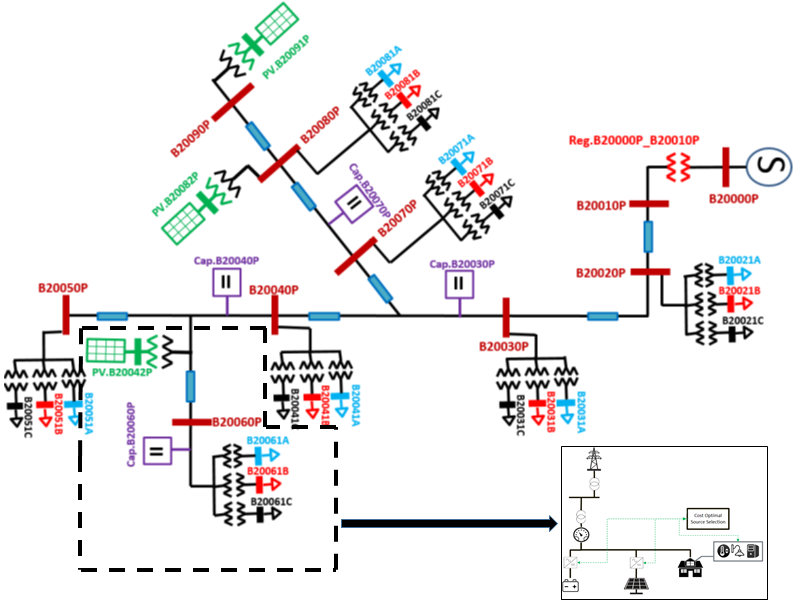
\includegraphics[width = \linewidth]{figs/A8/simulation_grid.png}
    \caption{Simulated system}
    \label{fig:simulation_grid}
\end{figure}


\begin{equation}
\label{eq:R_ESS}
R_{ESS} = \dfrac{ES_{tot}}{Cyc\cdot ES_{Cap}\cdot DoD\cdot \eta_{r}},
\end{equation}

where $ES_{tot}$ is the total cost of the ES system, $DoD$ is the desired depth-of-discharge of the ES system, $Cyc$ is the total number of cycles under warranty at depth-of-discharge, $ES_{Cap}$ is the total energy capacity of the ES system, and $\eta_r$ is the round-trip efficiency of the system. The data used to calculate the $R_{ESS}$ price used in the study were obtained from publicly available data on a commercial ES solution \cite{tesla_powerpack_2018}. 

%%%%%%%%PV%%%%%%%%%%%%%%%%%%%%%%%%%%%%%%%%%%%
\begin{table}[!ht]
%\normalsize
%\renewcommand{\arraystretch}{1}
\caption{PV System Specifications}
\label{tab:solar_pv}
\centering
    \begin{tabular}{ | l | p{3cm} | }
    \hline
    \textbf{PV System Parameters} & \textbf{Value} \\ \hline
    PV Panels Rating (\(P_{PV}\)) & 875 kW  \\ \hline
    Inverter Rating (\(S_{PV}\)) & 900 kVA \\ \hline
    Power Factor Range (\(pf_{PV}\)) & 0.8-1.0  \\ \hline
    Max. Reactive Power (\(\overline{Q_{PV}}\)) & 540 kVAR \\ \hline
    Min. Reactive Power (\(\underline{Q_{PV}}\)) & -540 kVAR \\ \hline
    LCOE (\(r_{PV}\)) & 2.51 c/kWh \\ \hline
    \end{tabular}
    \begin{tabular}{l}
    \end{tabular}
\end{table}
%%%%%%%%PV%%%%%%%%%%%%%%%%%%%%%%%%%%%%%%%%%%%


%%%%%%%%ES%%%%%%%%%%%%%%%%%%%%%%%%%%%%%%%%%%%
\begin{table}[!ht]
%\normalsize
%\renewcommand{\arraystretch}{1}
\caption{Energy Storage (ES) System Specifications}
\label{tab:es}
\centering
    \begin{tabular}{ | l | p{3cm} | p{3cm} | }
    \hline
    \textbf{ES System Parameters} & \textbf{Value} \\ \hline
    ES Rating (\(P_{ES}\)) & 750 kW  \\ \hline
    Inverter Rating (\(S_{ES}\)) & 750 kVA \\ \hline
    Max. State of Charge  (\(\overline{SOC_{ES}}\)) & 2190 kWh \\ \hline
    Min. State of Charge  (\(\underline{SOC_{ES}}\)) & 219 kWh \\ \hline
    Power Factor Range (\(pf_{ES}\)) & 0.8-1.0  \\ \hline
    Max. Reactive Power (\(\overline{Q_{ES}}\)) & 450 kVAR \\ \hline
    Min. Reactive Power (\(\underline{Q_{ES}}\)) & -450 kVAR \\ \hline
    LCOE (\(r_{ES}\)) & 12.3 c/kWh \\ \hline
    \end{tabular}
\end{table}
%%%%%%%%ES%%%%%%%%%%%%%%%%%%%%%%%%%%%%%%%%%%%

Fig. \ref{fig:LOAD_PROFILE_8} shows the load profile of the system for eight days with average, minimum, and maximum load values. To generate the RTP profile, Locational Based Marginal Pricing (LBMP) data were collected from the New York Independent System Operator (NYISO) \cite{NYISO2017}. The collected LBMPO was combined with the time of use (ToU) prices available at Tallahassee to generate an RTP for the proposed test cases. Another price profile was collected from the PG\&E peak day pricing scheme \cite{pgne}. Both profiles were used as RTP profiles to validate the algorithm under different pricing schemes. Fig. \ref{fig:RTP_PROFILE_8} shows the real-time price (RTP) profiles used for testing the proposed system. The solid lines represent the price profile collected from NYISO and the dashed lines represent the price profile collected from PG\&E. The eight-day PV and load profile used for the test system was collected from the SUNGRIN project and scaled to fit the ratings of the PV described in Table \ref{tab:solar_pv}. Fig. \ref{fig:PV_PROFILE_8} shows the eight-day PV profile used.

\begin{figure}[!ht]
    \centering
    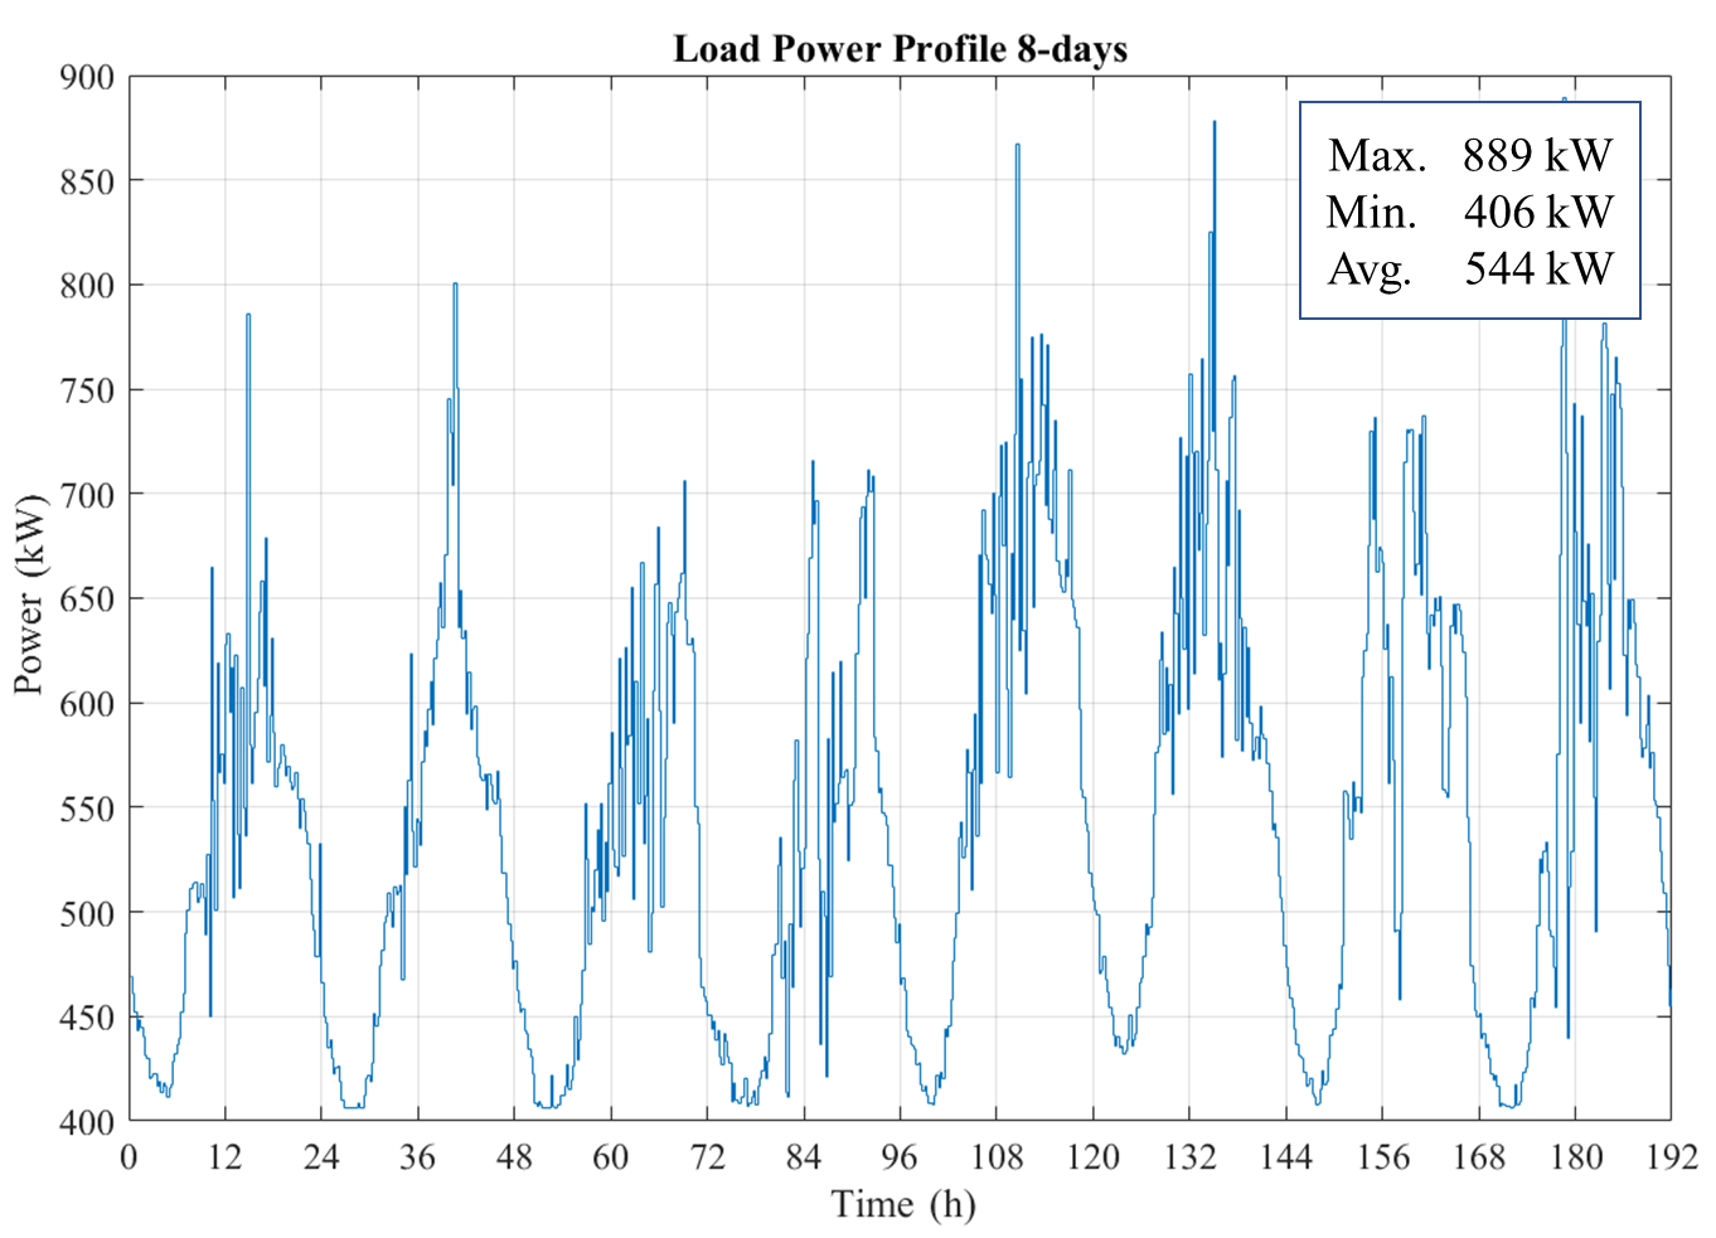
\includegraphics[width = \linewidth]{figs/A8/loadprofile.png}
    \caption{Eight day load profile}
    \label{fig:LOAD_PROFILE_8}
\end{figure}

\begin{figure}[!ht]
    \centering
    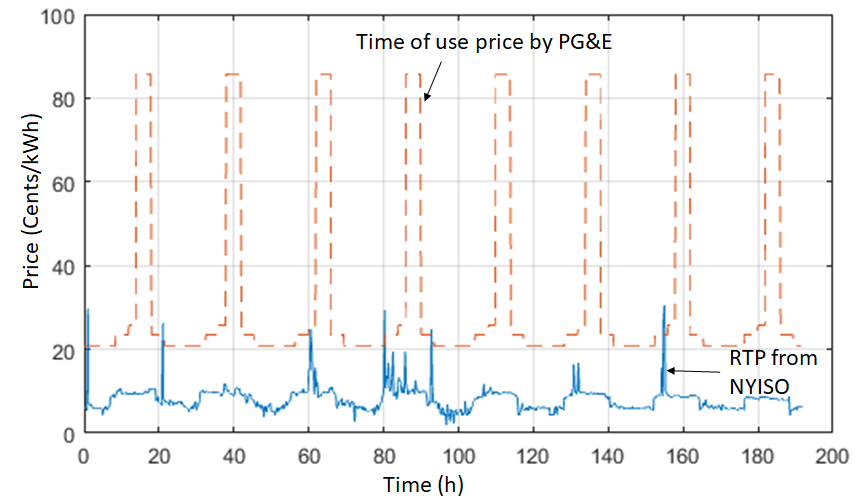
\includegraphics[width = \linewidth]{figs/A8/Price_profiles.png}
    \caption{Eight day RTP profile NYISO}
    \label{fig:RTP_PROFILE_8}
\end{figure}

% \begin{figure}[!ht]
%     \centering
%     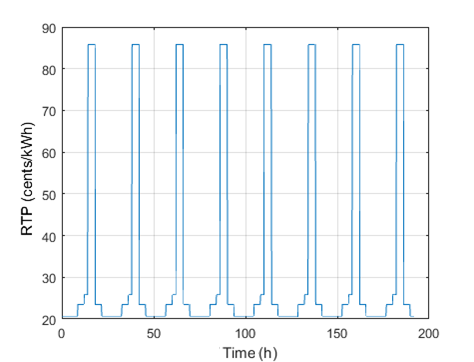
\includegraphics[width = \linewidth]{figs/PGNE_PRICE.png}
%     \caption{Eight day RTP profile PG\&E}
%     \label{fig:PGNE_PRICE}
% \end{figure}


\begin{figure}[!ht]
    \centering
    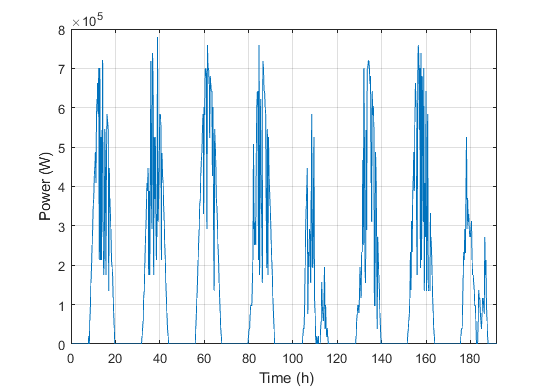
\includegraphics[width = \linewidth]{figs/A8/PV_PROFILE.png}
    \caption{Eight day PV profile}
    \label{fig:PV_PROFILE_8}
\end{figure}




\section{Offline simulation and results} \label{OFF}
The system described in Section \ref{sys} is modeled and simulated in MATLAB\textsuperscript{\textregistered} Simulink\textsuperscript{\textregistered} using the Simscape Power Systems\textsuperscript{TM} toolbox in phasor domain for the Offline simulation. The A* based ESM is run using the described data, and the results are fed in as an open loop control to a Simulink model for phasor simulation. In the test cases, the energy management problem is formulated according to the formulation discussed in Section \ref{formulation}. The  SOC of the ESS is discretized in steps of 2\%, and the SOC is limited between  94\%  and  10\%. The time step and the control horizon chosen is 15 minutes. The ES is allowed to charge or discharge a maximum of 8\% of its total capacity during one time-step. The 8\% limitation is set based on the power specifications discussed in table \ref{tab:es}. The A* search runs every 15 minutes considering a 24 hours (96 time-steps) prediction horizon. The performance of the A* based ESM is compared against two sample base test cases. The base test cases are the following:

\begin{enumerate}
\item \textbf{Case 1:} Charging the ES from 2 AM to 5 AM, Discharging the ES from 7 PM to 11 PM

\item \textbf{Case 2:} Charging from the ES 11 AM to 2 PM, Discharging the ES from 7 PM to 11 PM
\end{enumerate}

All the test cases are run under two different scenarios. The scenario I considers Net Metering Scheme and  Scenarios II considers different prices for buying and selling energy. 

\subsection{Scenario I: Net Metering} \label{netmeter}
In this scenario, the A* based EMS is compared against the two base test cases considering net metering. The NYISO RTP scheme shown in Fig. \ref{fig:RTP_PROFILE_8} is used for this comparison. The price of energy storage is chosen as 12.6 \cent/kWh. This price is calculated based on the specifications of the Tesla Powerpack \cite{tesla_powerpack_2018}.

Fig. \ref{fig:SBMPO_COMP_1_day} shows a zoomed view of the first day of the 7-day simulation for the A* based EMS. The solid black line in the figure represents the SOC of the energy storage, and the dotted red line represents the RTP. The dashed blue line represents the apparent demand. The left vertical axis of the graph represents the RTP of energy and the SOC of the ES. The right vertical axis represents the kWh apparent demand (actual demand - PV generation) of the system. A negative apparent demand represents excess energy from the local generation after fulfilling the local demand. The horizontal axis represents time in hours. The arrows with the numbers are showing specific points of the figure that are explained next, based on the behavior of the EMS. As observed in Fig. \ref{fig:SBMPO_COMP_1_day}, there are two peaks in price at the points 1 and 3 throughout the 24 hours window of operation. The ESM accurately anticipates the price peak in point 1 and charges the energy storage using the grid just before the peak occurs, and discharges during the price peak at point 1. It can be seen that during the peak, the apparent demand was positive and the lowest available price for grid energy was available just before the peak. The algorithm also anticipates the next price peak at point 3 based on forecasted data and prepares the ES to discharge at that price peak by charging at the lowest RTP period at point 2. Although, there is excess generation available from the PV in between point 2 and point 3 the opportunity cost of using the PV to charge the ES will be equal to the RTP due to net metering. So, in this case, the algorithm behaves as expected and uses the lowest possible RTP period to charge the ES and discharges during the price period when there is a high enough price peak to justify the use of the energy storage.

\begin{figure}[!ht]
    \centering
    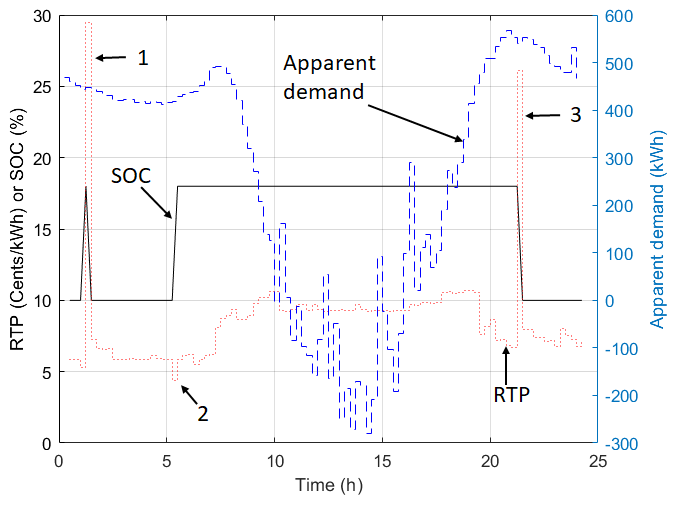
\includegraphics[width = 0.7\linewidth]{figs/A8/SBMPO_COMP_1_day.png}
    \caption{First day EMS response for net metering comparison case}
    \label{fig:SBMPO_COMP_1_day}
\end{figure}

Fig. \ref{fig:SBMPO_COMP_10_12} shows the response of the A*-based EMS in a seven days run used in the same microgrid system.  It can be seen from the figure that the A*-based ESM is following the same behavior displayed in Fig. \ref{fig:SBMPO_COMP_1_day}. It is taking advantage of the lowest energy price before a price peak appears in its prediction horizon, and charging the energy storage in order to discharge it when there is a high enough price peak. The total cost of operation for the A*-based ESM for the seven day period is shown in Table \ref{tab:Cost1}

\begin{table}[htb]
\caption{Seven day Cost for the three cases (net metering)}
\centering
\label{tab:Cost1}
\begin{tabular}{|l|l|}
\hline
Case1 & \$7,086 \\ \hline
Case2 & \$8,601 \\ \hline
A* Case & \$4,861 \\ \hline
A* Case \% savings (Case1) & 31.40\% \\ \hline
A* Case \% savings (Case2) & 43.48\% \\ \hline

\end{tabular}
\end{table}

\begin{figure}[!ht]
    \centering
    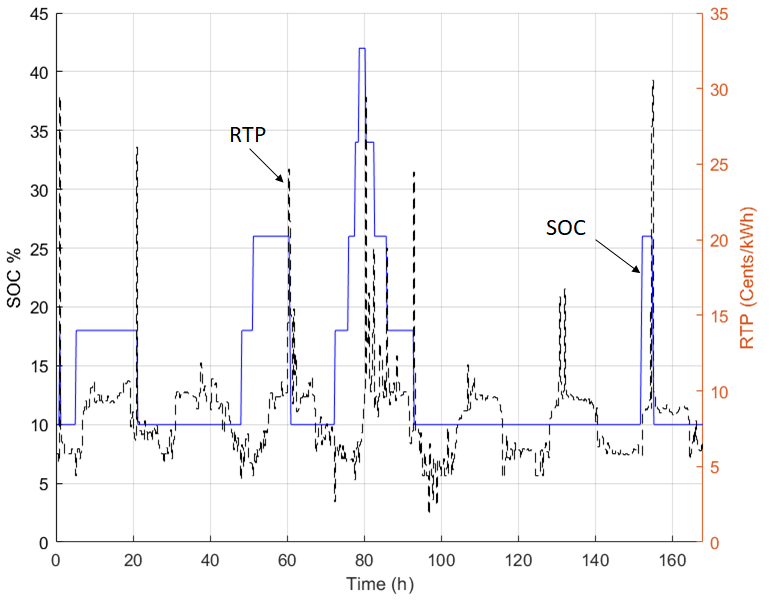
\includegraphics[width = 0.7\linewidth]{figs/A8/SBMPO_COMP_10_12.png}
    \caption{Full 7 day EMS response for net metering comparison case}
    \label{fig:SBMPO_COMP_10_12}
\end{figure}

\subsection{Scenario II: Buying and Selling Prices are Different}
In this scenario, the proposed algorithm is tested against the two base test cases using different price for selling power back to the grid. The cases 1 and 2 are previously fixed standard control strategies based on predefined charging and discharging of the energy storage mentioned before. The only difference is that the buying and selling price of energy from the grid is not the RTP. It is considered that the consumer is only allowed to sell power back to the grid at a rate of 4 cents/kWh.

Fig. \ref{fig:VAR_1_day_example} shows the 1-day test result for the A*-based EMS considering the RTP scheme shown in Fig. \ref{fig:RTP_PROFILE_8} for buying power and considering a sell-back price of 4 cents/kWh. The other system parameters are kept the same as the system used in the previous scenario. As seen in Fig. \ref{fig:VAR_1_day_example}, there are two peaks in price at the points 1 and 3 throughout the 24-hour window of operation. The ESM correctly anticipates the peak at point 1 and charges the energy storage using the grid just before the peak occurs and discharges during the price peak at point 1, similar to the behavior observed in the previous scenario. The next price peak is at point 3, and the lowest price for grid power available for charging the storage is at point 4. In case of a net metering scheme, point 4 would have been the best time to charge the ES in order to discharge it during the next price peak. However, since a sell-back price of 4 cents/kWh is being considered, this is no longer the case. The price 4 cents/kWh is lower than the price of buying grid energy at point 4. So the A*-based EMS takes into account that the opportunity cost for using power during point 2 instead of selling it back to the grid is 4 cents/kWh and decides to charge the ES during point 2 when there is additional local generation available. This behavior demonstrates that the A*-based ESM can use the forecasted knowledge of the future demand and RTP together to automatically decide the best moments to operate the energy storage depending on different pricing schemes.

 \begin{figure}[!ht]
    \centering
    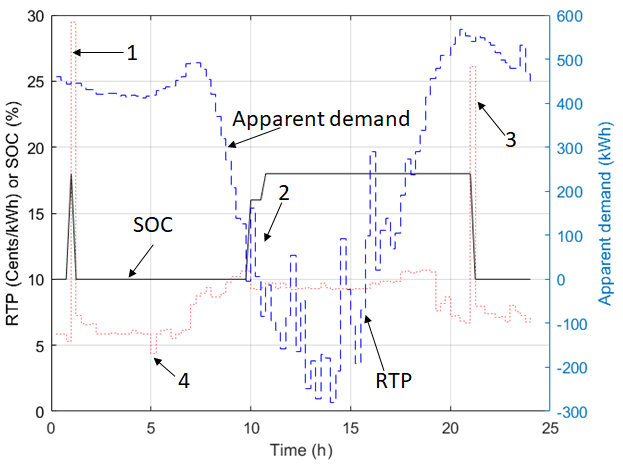
\includegraphics[width = 0.7\linewidth]{figs/A8/VAR_1_day_example.png}
    \caption{1 day EMS response considering NYISO price and 4 centes/kWh sellback price}
    \label{fig:VAR_1_day_example}
\end{figure}

Fig. \ref{fig:VAR_10_12_4} shows the 7-day test result for the tested microgrid considering the RTP shown in Fig. \ref{fig:RTP_PROFILE_8} and a sell-back price of 4 cents/kWh. Fig. \ref{fig:PG_VAR_10_12_4} show the ESM operation for the PG\&E profile shown in Fig. \ref{fig:RTP_PROFILE_8} considering 4 cents/kWh sell-back price. It can be observed from the 7-day cases, that the A*-based ESM shows behavior similar to the behavior seen in  Fig. \ref{fig:VAR_1_day_example}. The ESM scheme was also tested considering a sell-back price of 30\% of RTP for both the NYISO and PG\&E price profiles. The costs for the different conditions considered in the three cases are shown in Table \ref{tab:Cost}. Depending on the test case evaluated, the A* based ESM shows substantial cost savings of around 6.93\% to 41.79\%. 

 \begin{figure}[!ht]
    \centering
    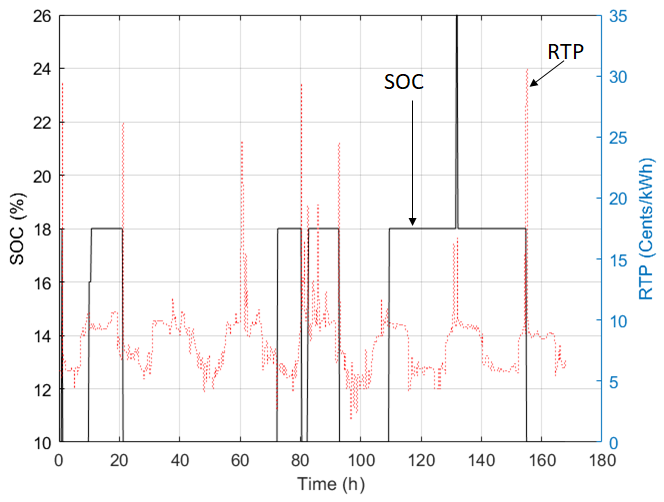
\includegraphics[width = 0.7\linewidth]{figs/A8/VAR_10_12_4.png}
    \caption{7 day EMS response considering NYISO price and 4 centes/kWh sell back price}
    \label{fig:VAR_10_12_4}
\end{figure}

%  \begin{figure}[!ht]
%     \centering
%     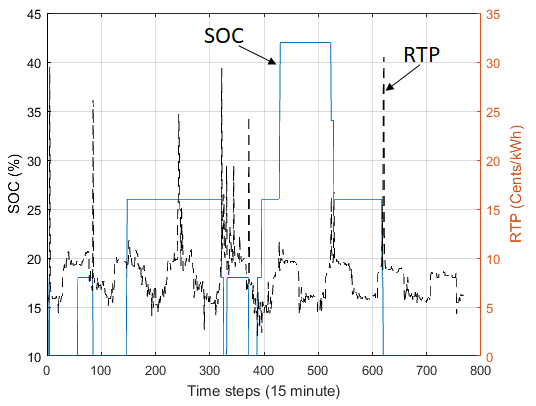
\includegraphics[width = \linewidth]{figs/VAR_10_12_30rtp.png}
%     \caption{7 day EMS response considering NYISO price and 30\% of RTP sell back price}
%     \label{fig:VAR_10_12_30rtp}
% \end{figure}

 \begin{figure}[!ht]
    \centering
    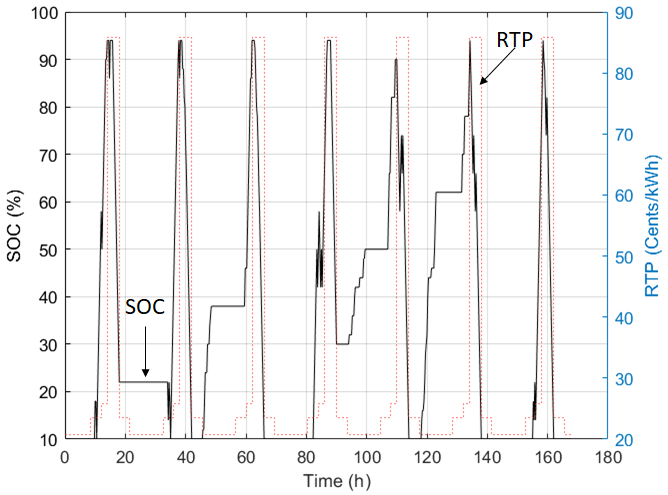
\includegraphics[width = 0.7\linewidth]{figs/A8/PG_VAR_10_12_4.png}
    \caption{7 day EMS response considering PG\&E price and 4 centes/kWh sell back price}
    \label{fig:PG_VAR_10_12_4}
\end{figure}

%  \begin{figure}[!ht]
%     \centering
%     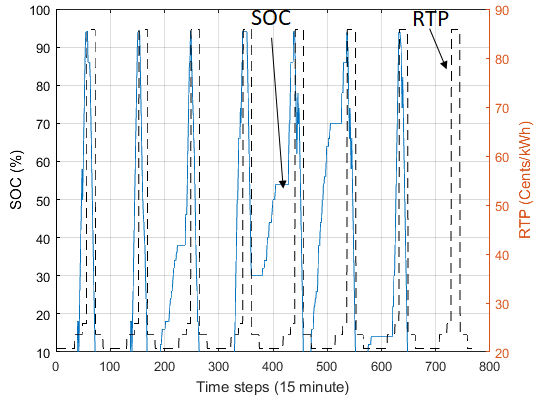
\includegraphics[width = \linewidth]{figs/PG_VAR_10_12_30rtp.png}
%     \caption{7 day EMS response considering PG\&E price and 30\% of RTP sell back price}
%     \label{fig:PG_VAR_10_12_30rtp}
% \end{figure}


%%%%%%%%CSOT%%%%%%%%%%%%%%%%%%%%%%%%%%%%%%%%%%%
\begin{table}[htb]
%\normalsize
%\renewcommand{\arraystretch}{1}
\caption{Seven day Cost for the three cases (different sell price)}
\label{tab:Cost}
\centering

\begin{tabular}{l|l|l|l|l|}
\cline{2-5}
                            & \multicolumn{2}{l|}{4 cents/kWh} & \multicolumn{2}{l|}{30\% RTP}   \\ \cline{2-5} 
                            & NYISO           & PG\&E          & NYISO          & PG\&E          \\ \hline
\multicolumn{1}{|l|}{Case1 cost} & \$8,265  & \$19,396 & \$8,314 & \$19,109 \\ \hline
\multicolumn{1}{|l|}{Case2 cost} & \$8,8606  & \$19,633 & \$8,895 & \$19,407 \\ \hline
\multicolumn{1}{|l|}{A* Case cost} & \$5,329  & \$18,051 & \$5,178 & \$17,106 \\ \hline
\multicolumn{1}{|l|}{A* Case \% savings (Case1)} & 35.52\%         & 6.93\%         & 37.72\%        & 10.84\%        \\ \hline
\multicolumn{1}{|l|}{A* Case \% savings (Case2)} & 39.85\%         & 8.08\%         & 41.79\%        & 11.86\%        \\ \hline
\end{tabular}

\end{table}
%%%%%%%%CSOT%%%%%%%%%%%%%%%%%%%%%%%%%%%%%%%%%%%%%%%%%%%

%%%%%%%%COMPARE_COST%%%%%%%%%%%%%%%%%%%%%%%%%%%%%%%%%%%
% \begin{table}[htb]
% %\normalsize
% %\renewcommand{\arraystretch}{1}
% \caption{Case 3 savings compared to other cases (7 days)}
% \label{tab:Cost_comp}
% \centering
% \begin{tabular}{l|l|l|l|l|}
% \cline{2-5}
%                             & \multicolumn{2}{l|}{4 cents/kWh} & \multicolumn{2}{l|}{30\% RTP}   \\ \cline{2-5} 
%                             & NYISO           & PG\&E          & NYISO          & PG\&E          \\ \hline
% \multicolumn{1}{|l|}{Case1} & 35.52\%         & 6.93\%         & 37.72\%        & 10.84\%        \\ \hline
% \multicolumn{1}{|l|}{Case2} & 39.85\%         & 8.08\%         & 41.79\%        & 11.86\%        \\ \hline
% \end{tabular}
% \end{table}
% %%%%%%%%COMPARE_COST%%%%%%%%%%%%%%%%%%%%%%%%%%%%%%%%%%%

\section{Real-time simulation and results} \label{RT}
A controller hardware in the loop (CHIL) simulation was set up to validate the algorithm in a real-time environment. 
The block layout of the CHIL simulation is shown in Fig. \ref{fig:RT_block}. The power system shown in Fig. \ref{fig:simulation_grid}, is simulated in real time in a digital real-time simulator (DRTS) with a time step of 50 ${\mu}s$. This system is modeled for detailed electromagnetic transient simulation unlike the phasor simulation model used in the offline simulation. The A* based ESM algorithm is implemented in Python 2.7 on a windows machine. The specifications of the machine are given in Table \ref{tab:PC}. The communication link between the DRTS and windows machine was established using TCP/IP. The DRTS sent the windows machine running the ESM the current PV generation ($P_{PV}(t)$), the current load ($P_load(t)$) and the current energy storage state of charge ($ES_{SOC}(t)$). The RTP, Load and PV prediction profiles are fed to the ESM by a pregenerated MATLAB formatted data (MAT) file. The current RTP is also provided by the MAT file. After receiving the current status and predicted profiles the ESM determines the power the ES should provide for the current time period ($P_{ES}(t)$) and sends it back to the DRTS. The actual CHIL setup is shown in Fig. \ref{fig:LAB_REAL}.

\begin{table}[htb]
\caption{Windows machine specification}
\label{tab:PC}
\centering
\begin{tabular}{|l|l|}
\hline
Operating system & Windows 10 Home 64-bit      \\ \hline
Processor        & Intel(R) Core(TM) i5-7300HQ \\ \hline
Memory           & 8192 MB RAM                 \\ \hline
\end{tabular}
\end{table}

\begin{figure}[!ht]
    \centering
    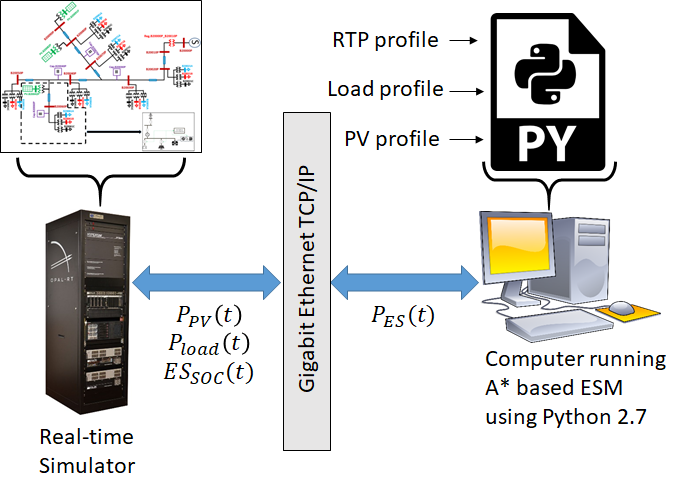
\includegraphics[width = 0.5\linewidth]{figs/A8/RT_block.png}
    \caption{Block layout of the CHIL setup}
    \label{fig:RT_block}
\end{figure}

\begin{figure}[!ht]
    \centering
    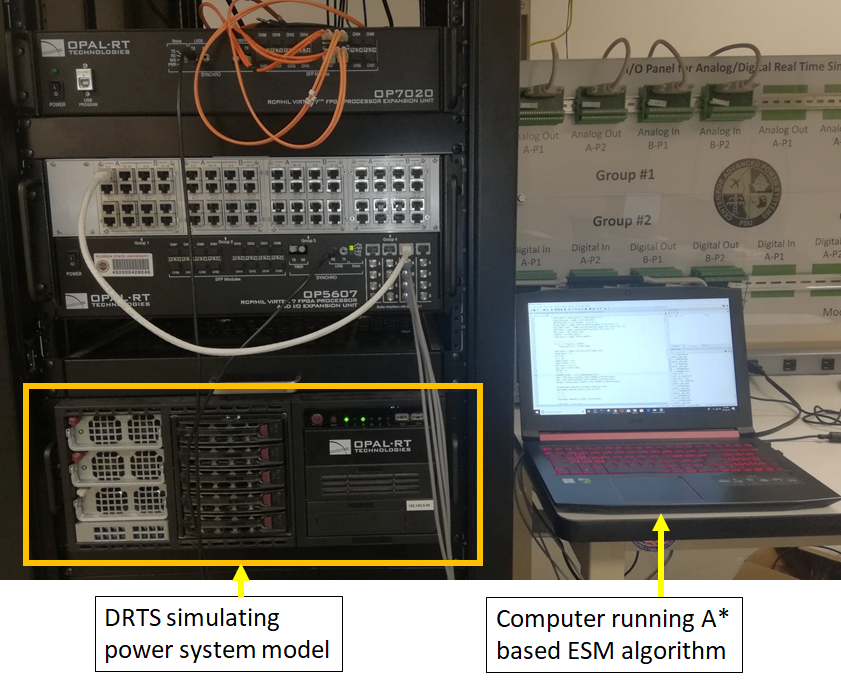
\includegraphics[width = 0.5\linewidth]{figs/A8/LAB_REAL.png}
    \caption{Actual CHIL setup}
    \label{fig:LAB_REAL}
\end{figure}

For the CHIL simulation, the ESM algorithm was set up according to the setup described in Section \ref{OFF}. The simulation was run for 50 hours (200 time steps) in real-time. Fig. \ref{fig:RT_TESTING} shows the real-time and the offline simulation results for the 50-hour run. It can be seen that the real-time simulation result shown by the dotted lines follows the off-line simulation result shown by the solid line. The results are similar to the first two days of Fig. \ref{fig:SBMPO_COMP_10_12} as expected. The comparison of the real-time and offline cost savings of the algorithm is shown in table \ref{tab:rt_cost}. It can be seen from the table that the real-time cost savings are comparable to the offline results.

\begin{figure}[!ht]
    \centering
    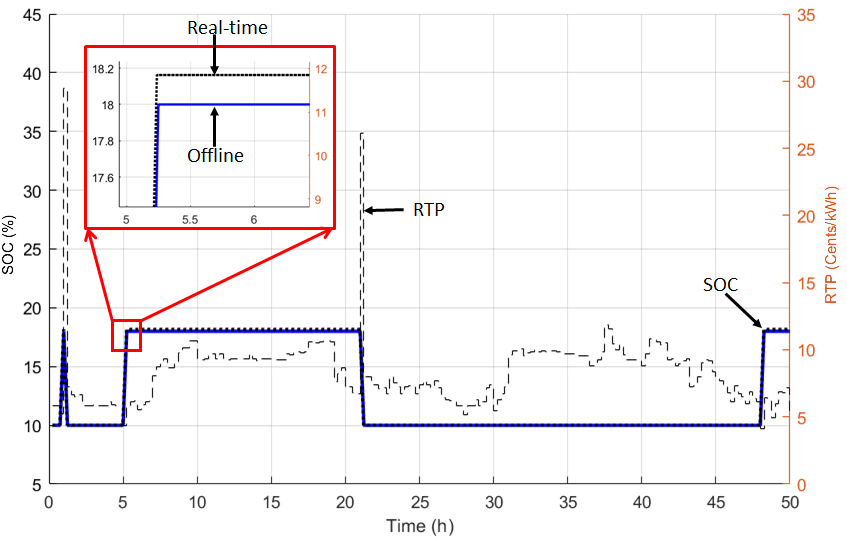
\includegraphics[width = 0.5\linewidth]{figs/A8/RT_TESTING.png}
    \caption{Real-time vs offline result (50  hours)}
    \label{fig:RT_TESTING}
\end{figure}

\begin{table}[htb]
\centering
\caption{Real-time simulation cost (48 hours)}
\label{tab:rt_cost}
\begin{tabular}{l|l|l|l|}
\cline{2-4}
                                          & Real-time & Offline & Difference \\ \hline
\multicolumn{1}{|l|}{Case1}               & \$1,662   & \$1,579 & 4.99\%     \\ \hline
\multicolumn{1}{|l|}{Cas2}                & \$1,713   & \$1,628 & 4.96\%     \\ \hline
\multicolumn{1}{|l|}{A* Case}             & \$1,345   & \$1,286 & 4.39\%     \\ \hline
\multicolumn{1}{|l|}{A* savings (Case 1)} & 19.07\%   & 18.56\% & 0.52\%     \\ \hline
\multicolumn{1}{|l|}{A* savings (Case 2)} & 21.48\%   & 21.01\% & 0.48\%     \\ \hline
\end{tabular}
\end{table}